\documentclass[../hw.tex]{subfiles}

\begin{document}
\setcounter{section}{8}
\begin{center}
  \section*{Homework 8} \label{sec:homework8}
  \subsection*{Due 3/27}
\end{center}
\addcontentsline{toc}{section}{\nameref{sec:homework8}}
\hrule \vspace{10px}
\paragraph*{1.}
From Figure \ref{fig:hw8_1} we use cylindrical coordinates and define an infinitesimal mass element
$\dd{m}$ that `feels' two forces: the gravitational and centrifugal force (due to the noninertial
reference frame) which is balanced by the force normal to the surface. This assumes that the water
does not move in the noninertial frame.
\begin{figure}[ht]
    \centering
    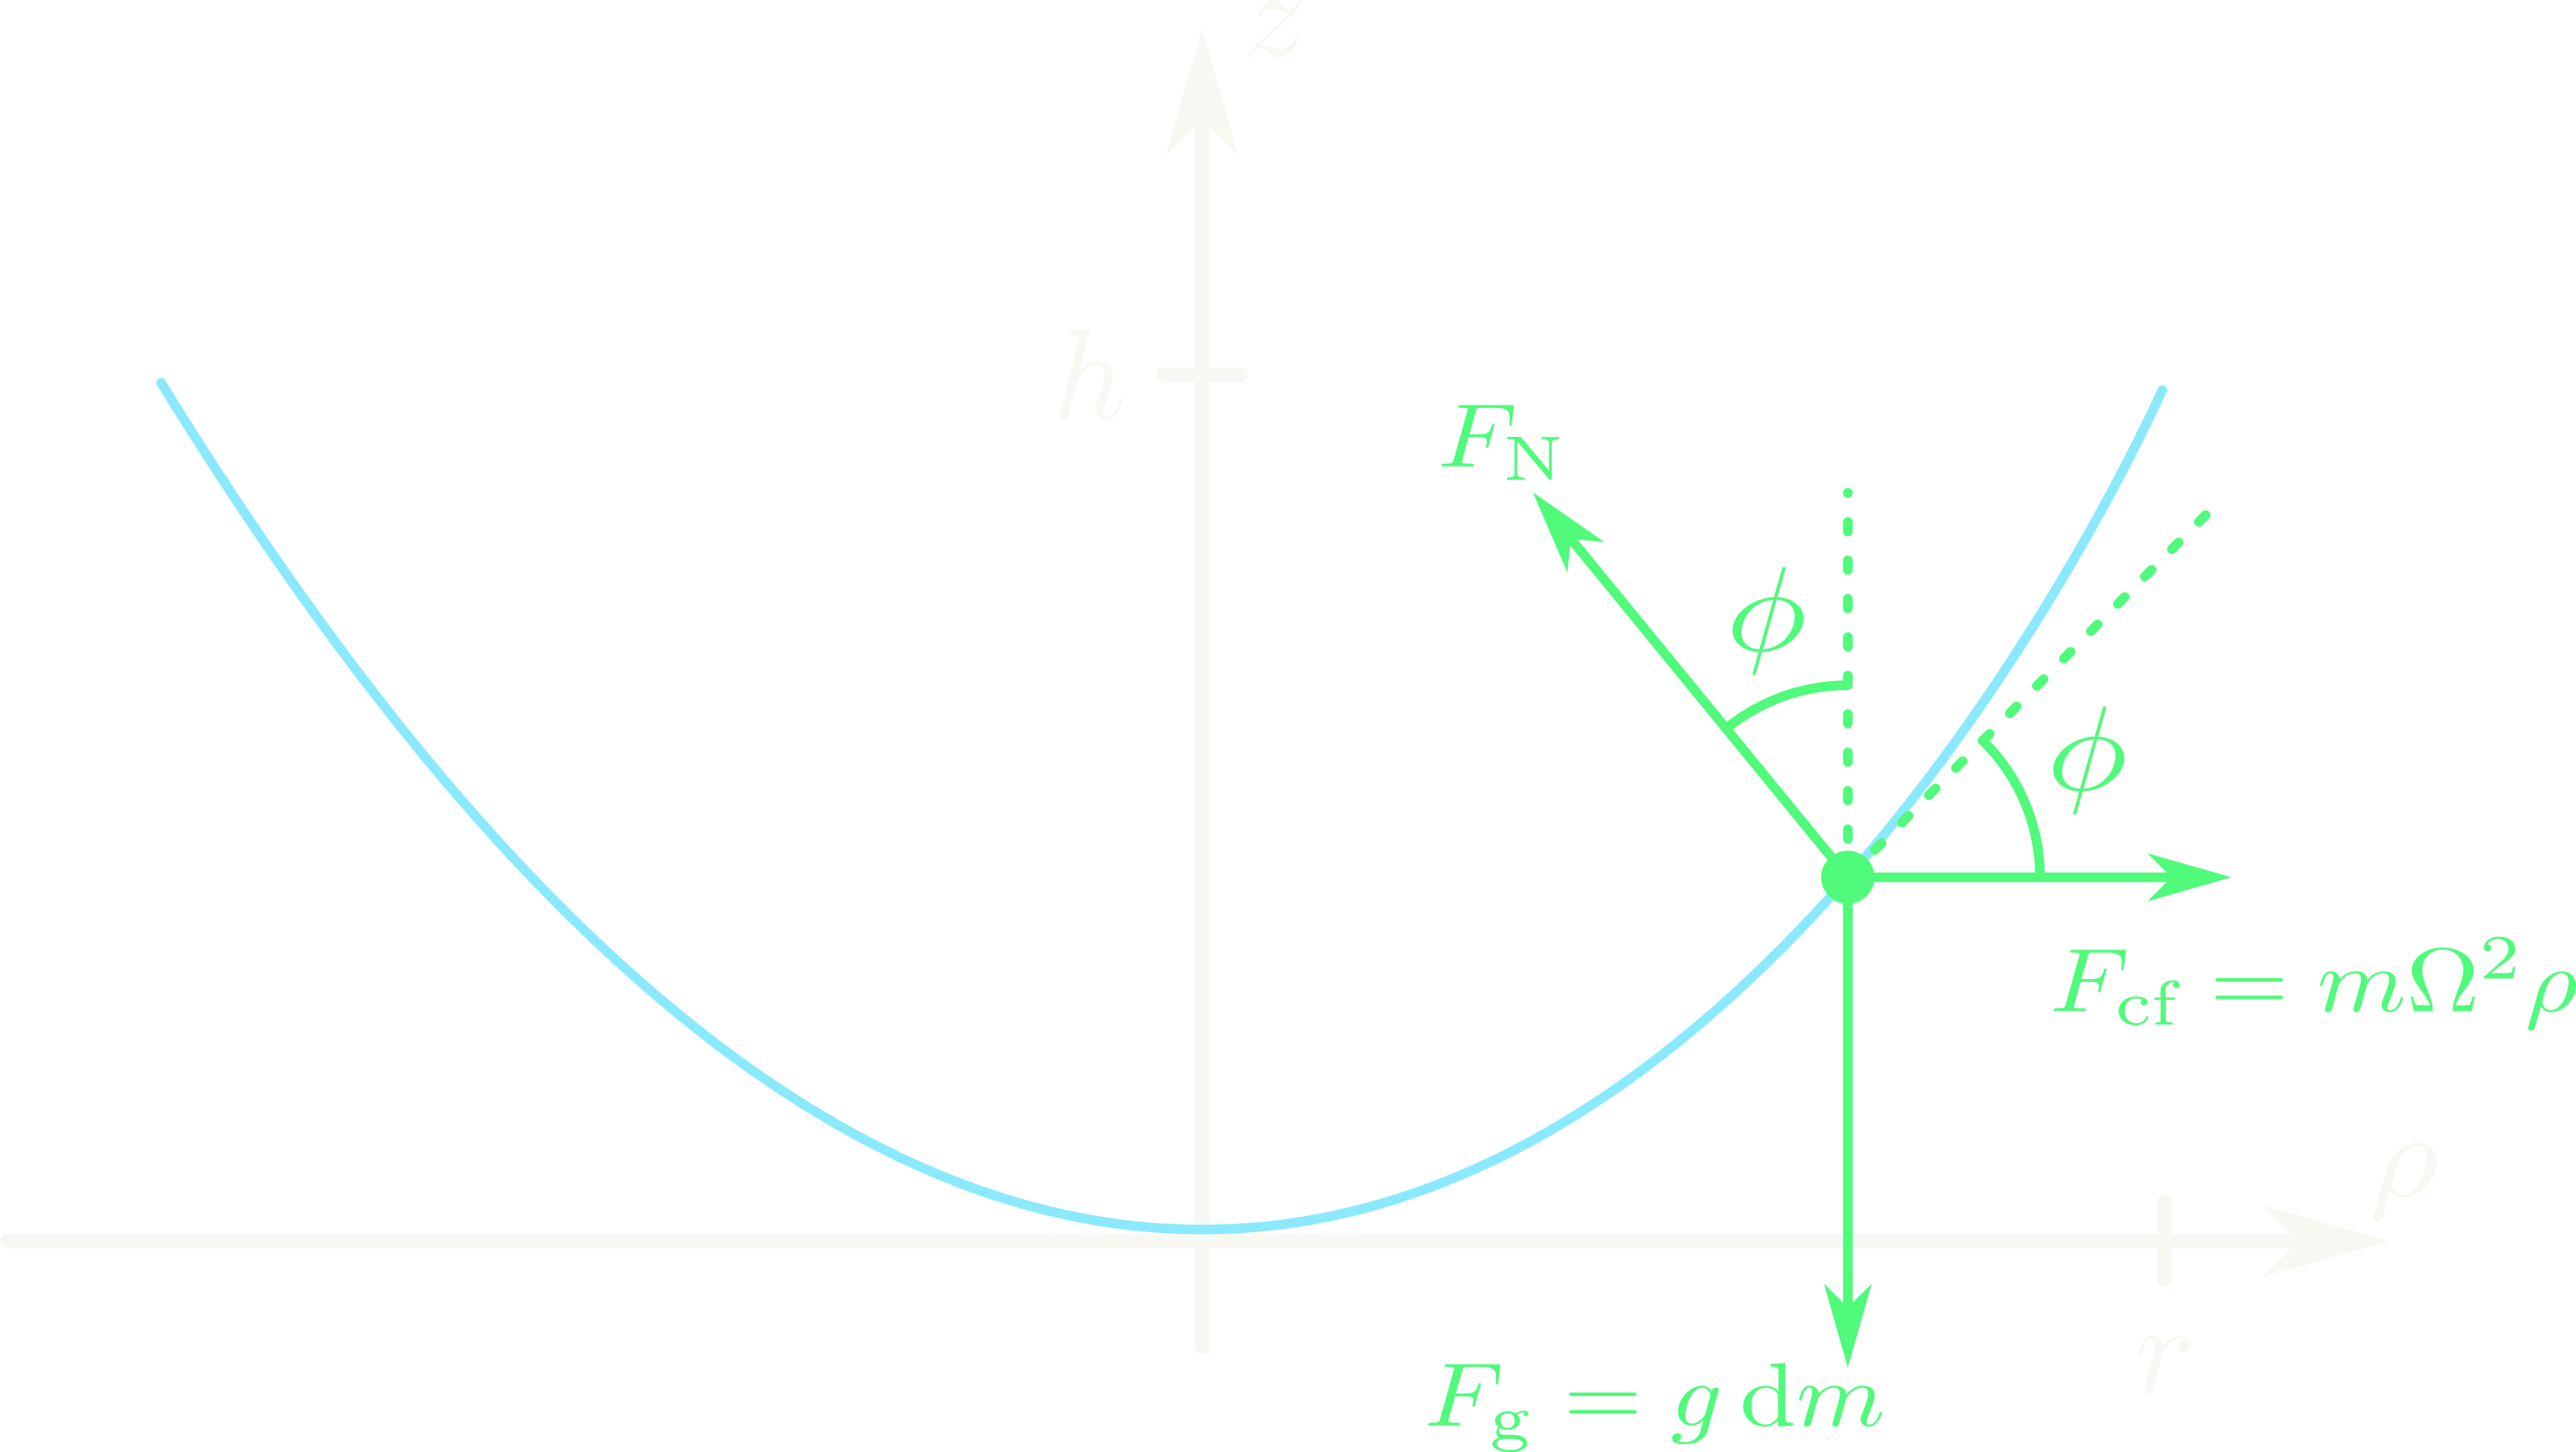
\includegraphics[width=0.5\textwidth]{hw8_1.png}
    \caption{A vertical cross section of the rotating bucket of water and its surface shape.}
    \label{fig:hw8_1}
\end{figure}

We can see that the angle with respect to the vertical is given by
\begin{align*}
    \tan \phi = \frac{F_{\text{g}}}{F_\text{cf}}
\end{align*}

\end{document}